\usetikzlibrary{calc}
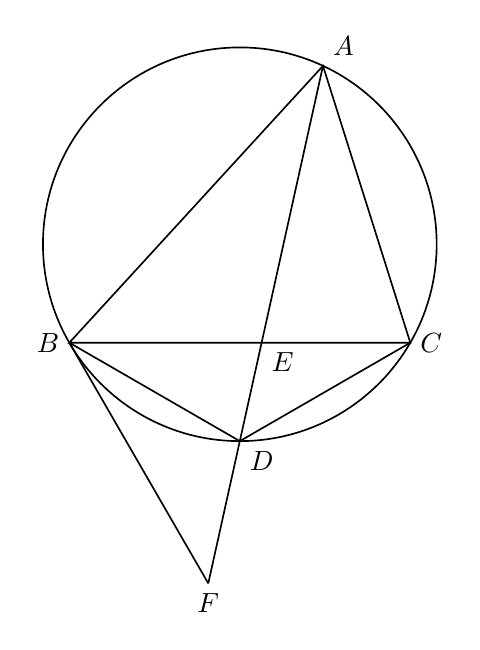
\begin{tikzpicture}[x=1cm,y=1cm,line width=.6pt,font=\normalsize]
\coordinate (A) at (1.0565,2.2658);
\coordinate (B) at (-2.1651,-1.25);
\coordinate (C) at (2.1651,-1.25);
\coordinate (D) at (0,-2.5);
\coordinate (E) at (0.2771,-1.25);
\coordinate (F) at (-0.4005,-4.3064);
\draw (0,0) circle[radius=2.5cm];
\draw (A)--(B)--(C)--cycle;
\draw (A)--(F);
\draw (B)--(F);
\draw (B)--(D);
\draw (D)--(C);
\node[above right] at (A) {$A$};
\node[left] at (B) {$B$};
\node[right] at (C) {$C$};
\node[below right] at (D) {$D$};
\node[below right] at (E) {$E$};
\node[below] at (F) {$F$};
\end{tikzpicture}
